\chapter{Aufgabenanalyse}
\section{Beschreibung Eingabedatei}

Die Eingabedatei muss UTF-8-kodiert sein;
anderenfalls wird eine Exception mit der Meldung „Eingabedatei ist nicht UTF-8 kodiert“ ausgelöst.
Die Datei gliedert sich in exakt drei Abschnitte: Zeitraum:, Einfallspunkte: und Kreuzungen:.
Jeder Abschnitt darf höchstens einmal vorkommen – doppelte Abschnitte führen zu einem Abbruch mit einer spezifischen Fehlermeldung.

Im Abschnitt Zeitraum: werden zwei Parameter erwartet: die Gesamtdauer der Simulation in Sekunden (maxTime) sowie die Taktfrequenz (clockrate),
also das Intervall in Sekunden, in dem Fahrzeuge generiert werden.
Beide Werte müssen positive Ganzzahlen sein. maxTime darf dabei 24 Stunden (86.400 Sekunden) nicht überschreiten.
Ein Eintrag wie z.,B. „50.0“ würde eine Fehlermeldung hervorrufen,
da Dezimalzahlen nicht erlaubt sind. Auch muss clockrate kleiner oder gleich maxTime sein.

Der Abschnitt Einfallspunkte: definiert Punkte,
an denen Fahrzeuge in das System eintreten.
Jede Zeile folgt dem Format Name X Y Ziel Takt. 
abei dürfen Namen maximal 100 Zeichen lang sein und nicht doppelt vorkommen.
Die Koordinaten X und Y müssen Gleitkommazahlen im Bereich von -1000 bis +1000 sein.
Zudem wird geprüft, dass kein Punkt näher als 0{,}1 Einheiten (entspricht 10 Metern) zu einem bereits definierten Punkt liegt.
Als Ziel wird eine Kreuzung angegeben, zu der das erste Fahrzeug weitergeleitet wird.
Der Takt bestimmt die Häufigkeit der Fahrzeuggenerierung in Sekunden und muss eine positive ganze Zahl sein.

Im Abschnitt Kreuzungen: wird jede Zeile im Format Name X Y Ziel1 Anteil1 Ziel2 Anteil2 ... erwartet.
Auch hier sind Namen auf 100 Zeichen begrenzt und dürfen nicht mehrfach vorkommen.
Die Ziel-Anteil-Paare müssen mindestens zweimal vorkommen,
wobei die Anzahl der Teile ungerade sein muss (wegen Name, X und Y zu Beginn).
Der Anteil (relative Wahrscheinlichkeit) muss als Dezimalzahl mit Punkt angegeben sein und zwischen $10^6$ und $10^{-6}$ liegen.
Auch hier dürfen Koordinaten nicht zu nahe beieinanderliegen.

Orte dürfen nicht gleichzeitig Einfallspunkte und Kreuzungen sein. Zudem müssen alle in Einfallspunkten oder Kreuzungen genannten Zielorte tatsächlich existieren – entweder als Kreuzung oder als anderer Einfallspunkt.

\section{Ausgabeanforderungen}

\section*{Ausgabe}

Für jede Simulation soll ein eigener Ordner angelegt werden,
dessen Name aus dem Präfix \texttt{output\_},
gefolgt vom Namen der Eingabedatei ohne Dateiendung, besteht. 
Beispielsweise wird die Ausgabe der Datei \texttt{Beispielhausen.txt} im Ordner \texttt{output\_Beispielhausen} gespeichert. 
Die Ausgabe des Programms besteht aus drei Dateien. 
Falls im Ordner bereits gleichnamige Dateien vorhanden sind, werden diese überschrieben.
Der neuerzeugte Ordner befindet sich auf gleicher Ebene, wie die ausführbare \texttt{.jar}.

\begin{enumerate}
  \item \textbf{Die Datei \texttt{Plan.txt}} beinhaltet die Koordinaten der Straßen. Jede Zeile besteht dabei aus vier Zahlen, die die $x$- und $y$-Koordinaten der Start- und Zielpunkte jeder Straße angeben.

  Für das folgende Beispiel hat die Datei \texttt{Plan.txt} folgenden Inhalt:

  \begin{verbatim}
0.0 0.0 1.0 0.0
1.0 0.0 2.0 0.0
2.0 0.0 3.0 0.0
0.0 0.0 0.0 1.0
0.0 1.0 0.0 2.0
0.0 2.0 0.0 3.0
0.0 3.0 1.0 3.0
1.0 3.0 2.0 3.0
2.0 3.0 3.0 3.0
3.0 3.0 3.0 2.0
3.0 2.0 3.0 1.0
3.0 1.0 3.0 0.0
3.0 0.0 4.0 0.0
4.0 0.0 5.0 0.0
4.0 0.0 4.0 1.0
4.0 1.0 4.0 2.0
4.0 2.0 4.0 3.0
4.0 3.0 5.0 3.0
5.0 3.0 5.0 2.0
5.0 2.0 5.0 1.0
5.0 1.0 5.0 0.0
  \end{verbatim}

  \item \textbf{Die Datei \texttt{Statistik.txt}} beinhaltet Statistiken zur Streckenauslastung jeder Straße. Es sollen zwei Werte pro Straße angegeben werden:
  \begin{itemize}
    \item \textit{Gesamtanzahl Fahrzeuge pro 100\,m}: Die Summe aller Fahrzeuge, die den jeweiligen Abschnitt befahren haben, normiert auf 100\,m.
    \item \textit{Maximale Anzahl Fahrzeuge pro 100\,m}: Die höchste gleichzeitige Anzahl an Fahrzeugen auf diesem Straßenabschnitt, ebenfalls normiert auf 100\,m.
  \end{itemize}

  \clearpage
  Beispielhafte Ausgabe der Datei \texttt{Statistik.txt}:

  \begin{verbatim}
Gesamtanzahl Fahrzeuge pro 100 m:
A -> B: 203.0
B -> A: 37.0
B -> C: 84.0
C -> B: 87.5
C -> D: 129.0
D -> C: 128.0
E -> F: 40.0
F -> E: 97.5
E -> G: 125.0
G -> E: 120.0

Maximale Anzahl Fahrzeuge pro 100 m:
A -> B: 10.0
B -> A: 2.0
B -> C: 6.0
C -> B: 2.0
C -> D: 8.0
D -> C: 8.0
E -> F: 2.0
F -> E: 4.75
E -> G: 8.75
G -> E: 4.0
  \end{verbatim}

Für die Ausgabe der Plan.txt und Statistik.txt wurde zusätzlich festgehalten, 
dass die Ausgabe sortiert nach den Namen der Orte (Einfallspunkte oder Kreuzungen) geschehen soll, sowie in den oben angegebenen Beispielen.

Das geschriebene Programm berechnet die Gesamtanzahl der Fahrzeuge wie folgt: 
Die Summe aller Fahrzeuge, die den jeweiligen Abschnitt befahren haben, normiert auf 100\,m. 
Mit dieser Methode lassen sich die Gesamtanzahlen aus den Beispielen nicht erreichen. 
Für die Beispiel-Gesamtanzahlen wurden vermutlich die Fahrzeuge kumuliert über alle Zeitschritte summiert und 
anschließend auf 100\,m normiert. 
Von dieser Methode wird abgewichen: Fahrzeuge werden auf einem Streckenabschnitt nur einmal gezählt. 
Die Gesamtanzahl sollte nicht von der gewählten allgemeinen Taktrate abhängen.

\clearpage

  \item \textbf{Die Datei \texttt{Fahrzeuge.txt}} enthält pro Zeitschritt alle sichtbaren Fahrzeuge mit:
  \begin{itemize}
    \item aktuellen Koordinaten,
    \item Koordinaten der nächsten Zielkreuzung,
    \item sowie fortlaufender Fahrzeug-ID.
  \end{itemize}

  Jeder Zeitschritt beginnt mit einer Zeile der Form:

  \begin{verbatim}
*** t = <Zeitpunkt>
  \end{verbatim}

  Beispielhafte Ausgabe:

  \begin{verbatim}
*** t = 0
4.0 2.0 4.0 1.0 0
4.0 0.0 4.0 1.0 1
...

*** t = 5
1.6215051939730939 3.0 4.0 1.0 0
1.626456506716547 3.0 4.0 1.0 1
...
  \end{verbatim}
\end{enumerate}

\subsection*{Visualisierung}

Die Simulation kann mit dem bereitgestellten Tool \texttt{Plot.py} visualisiert werden. Die Zielkreuzungen steuern die Fahrspurwahl (rechts oder links), und die Fahrzeug-ID bestimmt die Farbgebung.
Für jeden Zeitschritt wird eine PNG-Datei erstellt.


% \begin{figure}[h!]
%     \centering
%     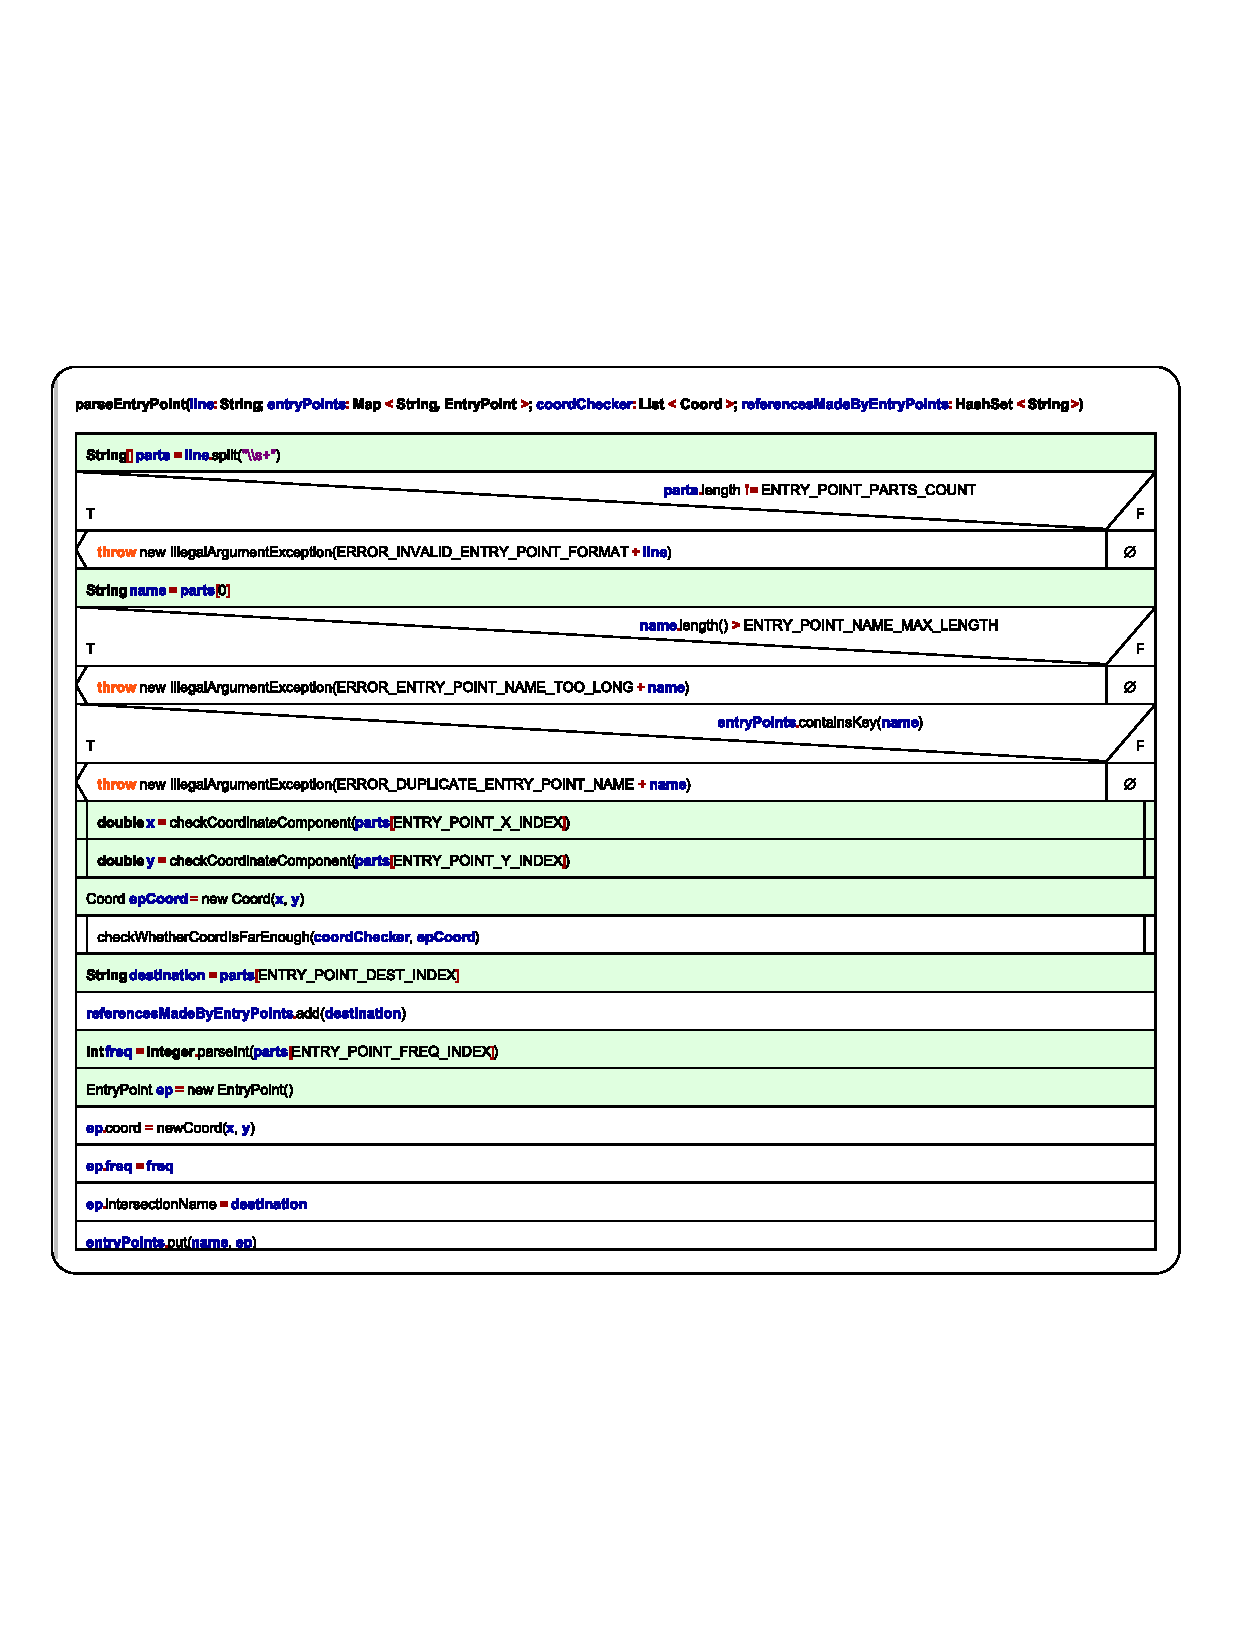
\includegraphics[width=0.8\textwidth]{nassis/TextFileReader/parseEntryPoint-4.pdf}
%     \caption{Example caption}
%     \label{fig:example}
% \end{figure}
